% Provenance (never printed): see sources/outline_sources.md (Year 2: fractional
% crystallisation, Bowen's series, compatible and incompatible elements, mixing and
% assimilation, layered intrusions).
% Curves from figdata/bachelor-2/differentiation.py (Bowen 1913 plagioclase loop, Rayleigh and
% equilibrium laws, Wilcox 1954 Paricutin analyses and mass balance, AFC closed form,
% Tegner et al. 2023 Skaergaard whole-rock data); exercise and problem values in the Book 4
% scratch calculator calc/ch08.py.
\chapter{Différenciation magmatique}\label{ch:b2:magmatic-differentiation}

Le 20 février 1943, un volcan commença à entrer en éruption dans l'ouest du Mexique, et
l'éruption dura neuf ans. Ses premières laves étaient des andésites basaltiques à \qty{55}{\percent}
de silice~; les dernières, de février 1952, étaient des andésites à un peu plus de
\qty{60}{\percent}. Le volcan, Parícutin, ne changea pas de source entre-temps, et ses laves furent
analysées une à une à mesure qu'elles sortaient. Le \omterm{def:b2:magma-emplacement:magma}{magma} situé sous lui se transforma
lui-même~: il fit croître des cristaux qu'il laissa sur place, et il dévora une partie
de la roche granitique environnante. Un \omterm{def:b2:magma-emplacement:magma}{magma} qui quitte le manteau sous forme de basalte peut
finir en rhyolite, et les roches qu'il laisse derrière lui sur son chemin gardent la trace
de la manière dont il s'y est pris. Ce chapitre suit un \omterm{def:b2:magma-emplacement:magma}{magma} pendant son refroidissement~: l'ordre
dans lequel les minéraux cristallisent, les lois qui décrivent comment les éléments majeurs et en traces
changent lorsque des cristaux sont retirés, les roches formées de ces cristaux, et ce qui se passe
quand le \omterm{def:b2:magma-emplacement:magma}{magma} absorbe un autre \omterm{def:b2:magma-emplacement:magma}{magma} ou la croûte.
% ledger: wilcox54:paricutin

\begin{recall}
\textbf{Du volume des classes 10 à 12}~: les roches magmatiques et leurs textures~; l'ordre dans lequel
les minéraux cristallisent à partir d'un \omterm{def:b2:magma-emplacement:magma}{magma} basaltique, l'olivine en premier et le quartz en dernier,
établi par les expériences de Bowen. \textbf{Du volume de chimie de deuxième année}~: diagrammes
de phases binaires, solutions solides et règle des leviers. \textbf{Du volume de première année}~:
le plagioclase, solution solide entre l'anorthite \ce{CaAl2Si2O8} et l'albite \ce{NaAlSi3O8}, et les
autres silicates des roches~; lames minces entre polariseurs croisés. \textbf{Du
\cref{ch:b2:elements-in-the-earth}}~: les \omterm{def:b2:elements-in-the-earth:partition}{coefficients de partage minéral--liquide} et global,
$\bar D = \sum_i x_i D_i$, les \omterm{def:b2:elements-in-the-earth:partition}{éléments compatibles} et incompatibles, les \omterm{def:b2:elements-in-the-earth:normalised}{diagrammes normalisés}
et l'\omterm{prop:b2:elements-in-the-earth:normalised}{anomalie en europium}. \textbf{Du \cref{ch:b2:isotope-geochemistry}}~: les rapports
isotopiques comme traceurs et l'\omterm{prop:b2:isotope-geochemistry:mixing}{hyperbole de mélange}. \textbf{Du
\cref{ch:b2:mantle-melting}}~: l'eutectique diopside--anorthite, la \omterm{def:b2:mantle-melting:peritectic}{fusion incongruente}, les diagrammes
ternaires et les \omterm{def:b2:mantle-melting:primary}{magmas primaires}.
\end{recall}

\section{Séquences de cristallisation}\label{sec:b2:magmatic-differentiation:sequences}

Un \omterm{def:b2:magma-emplacement:magma}{magma} basaltique ne cristallise pas tous ses minéraux à la fois. Bowen a établi par
l'expérience que l'olivine cristallise normalement en premier, entre 1200 et
\qty{1300}{\celsius}~; que le plagioclase riche en calcium commence à peu près en même temps que
le pyroxène~; et que le dernier liquide, riche en silice, donne du feldspath potassique, du quartz et
peut-être de la muscovite vers 750 à \qty{800}{\celsius}. Entre les deux, les minéraux mafiques
ne s'accumulent pas simplement~: chacun réagit avec le liquide pour donner le suivant.
% ledger: earle:bowen (Book 2), tulane:bowen (Book 2)

\begin{definition}[Suite réactionnelle de Bowen]\label{def:b2:magmatic-differentiation:bowen}
\emph{suite réactionnelle de Bowen}\index{suite réactionnelle de Bowen} est l'ordre dans lequel
les silicates courants cristallisent à partir d'un \omterm{def:b2:magma-emplacement:magma}{magma} basaltique en refroidissement, en deux branches
qui se rejoignent à la fin. Dans la \emph{branche discontinue}, chaque minéral mafique réagit avec le
liquide pour former un nouveau minéral d'une autre structure~: olivine, pyroxène, amphibole, biotite.
Dans la \emph{branche continue}, le plagioclase cristallise tout au long,
sa composition passant continûment du riche en calcium au riche en sodium. Le dernier liquide
cristallise du feldspath potassique, de la muscovite et
du quartz.
\end{definition}
% ledger: earle:bowen (Book 2)

\begin{omfigure}
\centering
\begin{tikzpicture}[font=\small, x=1cm, y=1cm,
  mn/.style={draw, rounded corners=2pt, fill=white, inner sep=3pt, minimum width=2.3cm,
             align=center}]
\draw[-{Stealth[length=4pt]}, thick, gray] (-1.3,0.3) -- (-1.3,-6.0);
\node[rotate=90, anchor=south, font=\scriptsize, gray] at (-1.4,-2.85) {température décroissante};
\node[anchor=east, font=\scriptsize] at (-1.5,0) {$\approx$ 1200--\qty{1300}{\celsius}};
\node[anchor=east, font=\scriptsize] at (-1.5,-5.6) {$\approx$ 750--\qty{800}{\celsius}};
\node[mn] (ol) at (1,0) {olivine};
\node[mn] (px) at (1,-1.4) {pyroxène};
\node[mn] (am) at (1,-2.8) {amphibole};
\node[mn] (bt) at (1,-4.2) {biotite};
\draw[-{Stealth[length=4pt]}, thick] (ol) -- (px);
\draw[-{Stealth[length=4pt]}, thick] (px) -- (am);
\draw[-{Stealth[length=4pt]}, thick] (am) -- (bt);
\node[font=\scriptsize, align=center] at (1,0.8) {branche discontinue\\(un nouveau minéral à chaque étape)};
\node[mn] (ca) at (6,-1.4) {plagioclase\\riche en calcium};
\node[mn] (na) at (6,-4.2) {plagioclase\\riche en sodium};
\fill[left color=white, right color=white, top color=orange!35, bottom color=orange!8]
  (5.75,-2.0) rectangle (6.25,-3.6);
\draw[-{Stealth[length=4pt]}, thick] (ca) -- (na);
\node[font=\scriptsize, align=center] at (6,0.8) {branche continue\\(un seul minéral, à composition variable)};
\node[mn, minimum width=7.2cm] (last) at (3.5,-5.6) {feldspath potassique, muscovite, quartz};
\draw[-{Stealth[length=4pt]}, thick] (bt) -- (bt|-last.north);
\draw[-{Stealth[length=4pt]}, thick] (na) -- (na|-last.north);
\end{tikzpicture}
\par\smallskip{\small \omterm{def:b2:magmatic-differentiation:bowen}{Suite réactionnelle de Bowen}. L'olivine et le plagioclase riche en calcium cristallisent
en premier à partir d'un \omterm{def:b2:magma-emplacement:magma}{magma} basaltique~; à gauche, chaque minéral mafique réagit avec le liquide pour donner
le suivant~; à droite, le plagioclase s'enrichit sans cesse en sodium~; le dernier liquide, riche en silice,
donne du feldspath potassique, de la muscovite et du quartz. Les températures sont des valeurs typiques
d'un \omterm{def:b2:magma-emplacement:magma}{magma} basaltique à basse pression.}
\end{omfigure}
% ledger: earle:bowen (Book 2)

Les deux branches correspondent aux deux types de diagramme de phases du
\cref{ch:b2:mantle-melting}. Une réaction discontinue est la \omterm{def:b2:mantle-melting:peritectic}{fusion incongruente} de l'enstatite
parcourue à l'envers~: des cristaux de forstérite réagissent avec un liquide plus riche en silice
pour donner de l'enstatite. La branche continue est une solution solide. Bowen l'a mesurée en 1913
sur des plagioclases de synthèse, en maintenant chaque composition à une température connue et en
cherchant le verre et les cristaux~: l'anorthite fond à \qty{1550}{\celsius}, l'albite vers
\qty{1100}{\celsius}, et chaque plagioclase intermédiaire fond sur un intervalle compris
entre une courbe inférieure, le solidus, et une courbe supérieure, le liquidus (la figure
ci-dessous).
% ledger: bowen13:plagioclase, bowen14:mgo-sio2

\begin{omfigure}
\centering
\begin{tikzpicture}
\begin{axis}[omrecord, width=0.78\linewidth, height=6.4cm,
  xmin=0, xmax=100, ymin=1050, ymax=1600,
  xlabel={anorthite (\unit{\percent}, molaire)}, ylabel={température (\unit{\celsius})},
  y tick label style={/pgf/number format/1000 sep={}}, unbounded coords=discard,
  tick label style={font=\scriptsize}, label style={font=\small}]
\addplot[very thick, black] table[x=an, y=T_liq] {figdata/out/bachelor-2-differentiation-plag-curve.dat};
\addplot[very thick, black, dashed] table[x=an, y=T_sol] {figdata/out/bachelor-2-differentiation-plag-curve.dat};
\addplot[only marks, mark=*, mark size=1.5pt, blue!70!black] table[x=an, y=T_liq] {figdata/out/bachelor-2-differentiation-plag-data.dat};
\addplot[only marks, mark=o, mark size=1.7pt, blue!70!black] table[x=an, y=T_sol] {figdata/out/bachelor-2-differentiation-plag-data.dat};
\draw[densely dotted, red!70!black, thick] (axis cs:50,1560) -- (axis cs:50,1287);
\draw[red!70!black, thick] (axis cs:50,1450) -- (axis cs:80.6,1450);
\draw[red!70!black, thick] (axis cs:33.3,1394) -- (axis cs:70.6,1394);
\draw[red!70!black, thick] (axis cs:13.9,1287) -- (axis cs:50,1287);
\addplot[only marks, mark=*, mark size=1.4pt, red!70!black] coordinates {(50,1450) (80.6,1450) (33.3,1394) (70.6,1394) (13.9,1287) (50,1287)};
\node[font=\scriptsize] at (axis cs:30,1530) {liquide};
\node[font=\scriptsize, align=center] at (axis cs:83,1200) {plagioclase\\(solution solide)};
\node[font=\scriptsize, anchor=west] at (axis cs:2,1430) {liquidus (trait plein)};
\node[font=\scriptsize, anchor=west] at (axis cs:42,1160) {solidus (tirets)};
\node[font=\scriptsize, anchor=south, red!70!black, fill=white, inner sep=1pt] at (axis cs:68,1452) {\qty{1450}{\celsius}};
\node[font=\scriptsize, anchor=north, red!70!black, fill=white, inner sep=1pt] at (axis cs:31,1284) {\qty{1287}{\celsius}};
\end{axis}
\end{tikzpicture}
\par\smallskip{\small Les feldspaths plagioclases à la pression atmosphérique, d'après les
expériences de trempe de Bowen (1913)~: début (cercles) et fin (points) de la fusion, avec des courbes
tracées à travers les mesures. En rouge, la \omterm{def:b2:magmatic-differentiation:crystallisation}{cristallisation à l'équilibre} d'un liquide à
\qty{50}{\percent} d'anorthite~: le premier cristal, à \qty{1450}{\celsius}, contient
\qty{81}{\percent} d'anorthite~; à \qty{1394}{\celsius}, des cristaux à \qty{71}{\percent} coexistent
avec un liquide à \qty{33}{\percent}~; le dernier liquide, à \qty{1287}{\celsius}, en contient
\qty{14}{\percent} (\cref{exo:b2:magmatic-differentiation:1}).}
\end{omfigure}
% ledger: bowen13:plagioclase

Un liquide qui cristallise une solution solide s'enrichit du composant qui fond à la plus
basse température~: le premier plagioclase d'un liquide à \qty{50}{\percent} d'anorthite
contient \qty{81}{\percent} d'anorthite, et le liquide évolue vers l'albite. La suite dépend
de savoir si les cristaux continuent à échanger avec le
liquide.

\begin{definition}[Cristallisation à l'équilibre et fractionnée]
\label{def:b2:magmatic-differentiation:crystallisation}
Dans la \emph{cristallisation à l'équilibre}\index{cristallisation à l'équilibre} les
cristaux restent en équilibre chimique avec la totalité du liquide jusqu'à la
fin, en se rééquilibrant à mesure que le liquide change~; le système finit avec la composition
qu'il avait au départ. Dans la \emph{cristallisation fractionnée}\index{cristallisation fractionnée}
chaque cristal, une fois formé, est retiré de la réaction avec le liquide, par
décantation, en étant plaqué sur les parois de la chambre, ou en étant recouvert par une
croissance ultérieure~; le liquide évolue alors comme si les cristaux avaient été retirés du
système.
\end{definition}

En \omterm{def:b2:magmatic-differentiation:crystallisation}{cristallisation à l'équilibre}, le plagioclase de la figure ci-dessus passe de
\qty{81}{\percent} à \qty{50}{\percent} d'anorthite en croissant, chaque cristal se rééquilibrant par
diffusion avec le liquide, et le dernier liquide disparaît au solidus, à
\qty{1287}{\celsius}. La diffusion dans les feldspaths est lente, et les cristaux naturels
la suivent rarement~: l'intérieur de chaque cristal est coupé du liquide, qui se comporte alors
comme dans la \omterm{def:b2:magmatic-differentiation:crystallisation}{cristallisation fractionnée} et peut atteindre des compositions proches de
l'albite. La figure de la dernière section de ce chapitre calcule les deux trajets.
% ledger: bowen13:plagioclase

\begin{definition}[Lignée de différenciation du liquide]\label{def:b2:magmatic-differentiation:lld}
La \emph{lignée de différenciation du liquide}\index{lignée de différenciation du liquide} d'un \omterm{def:b2:magma-emplacement:magma}{magma} est la
suite des compositions prises par son liquide au fur et à mesure qu'il cristallise, tracée sur un
diagramme de variation ou un diagramme de phases.
\end{definition}

Une \omterm{def:b2:magmatic-differentiation:lld}{lignée de différenciation du liquide} ne caractérise que le liquide. Les laves émises avec
des cristaux en suspension ne s'y trouvent pas exactement, et Wilcox, en étudiant les laves du
Parícutin, utilisa à la fois leurs analyses sur roche totale et les compositions de leur pâte, la partie
liquide, calculée en retirant les cristaux.
% ledger: wilcox54:groundmass

\section{Fractionnement par cristallisation des éléments majeurs}\label{sec:b2:magmatic-differentiation:majors}

Retirer des cristaux modifie la composition du liquide d'une façon simple et linéaire,
et l'outil le plus ancien pour la lire est le tracé de chaque oxyde en fonction de la silice.

\begin{definition}[Diagramme de Harker]\label{def:b2:magmatic-differentiation:harker}
Un \emph{diagramme de Harker}\index{diagramme de Harker} (diagramme de variation en silice) porte le
pourcentage massique de chaque oxyde d'une suite de roches apparentées en fonction de leur
pourcentage massique de \ce{SiO2}, un panneau par oxyde.
\end{definition}


Les laves du Parícutin présentent de telles tendances (les \omterm{def:b2:magmatic-differentiation:harker}{diagrammes de Harker} de la
proposition suivante)~: quand la silice augmente, la magnésie, la chaux et l'alumine diminuent, et la potasse
augmente. C'est ce que produirait le retrait d'olivine et de plagioclase~:
l'olivine retire la magnésie et le fer, le plagioclase la chaux et l'alumine, et tous deux laissent le liquide
plus riche en silice et en alcalins. Savoir si le retrait de minéraux connus peut rendre compte
quantitativement de ces tendances est une question de bilan de masse.

\begin{proposition}[Bilan de masse du retrait de cristaux]\label{prop:b2:magmatic-differentiation:lever}
Soit un \omterm{def:b2:magma-emplacement:magma}{magma} parent de composition $\mathbf p$ (un vecteur de fractions massiques d'oxydes)
qui cristallise des minéraux de compositions $\mathbf m_1, \dots, \mathbf m_k$ en masses
$x_1, \dots, x_k$ par unité de masse de parent, et soit $\mathbf d$ la composition
du liquide restant. Alors
\[
\mathbf p = \Big(1 - \sum_i x_i\Big)\mathbf d + \sum_i x_i \mathbf m_i .
\]
Pour un seul minéral, le parent se situe sur le segment droit joignant le liquide et le
minéral, sur tout diagramme de variation, et la fraction massique retirée vaut
$x = (p_j - d_j)/(m_j - d_j)$ pour tout oxyde $j$~: c'est la règle des leviers.
\end{proposition}

\begin{proof}
Chaque oxyde est conservé~: la masse $p_j$ de l'oxyde $j$ dans une unité de masse de parent finit
soit dans le liquide, de masse $1 - \sum_i x_i$ et de concentration $d_j$, soit dans les
minéraux. Écrire cela pour chaque $j$ donne l'équation vectorielle. Avec un seul minéral, elle
s'écrit $\mathbf p = (1-x)\mathbf d + x\mathbf m$, un point du segment joignant $\mathbf d$ à
$\mathbf m$ qui le divise dans le rapport $x : (1-x)$, sur n'importe quel couple d'axes~; résoudre
une composante donne $x$.
\end{proof}

\begin{omfigure}
\centering
\begin{tikzpicture}
\begin{groupplot}[group style={group size=2 by 2, horizontal sep=1.6cm, vertical sep=1.3cm},
  width=0.44\linewidth, height=4.3cm, omrecord, xmin=54.5, xmax=60.8,
  tick label style={font=\scriptsize}, label style={font=\small},
  xtick={55,56,57,58,59,60}]
\nextgroupplot[ylabel={\ce{MgO} (\unit{\percent})}, ymin=3.2, ymax=6.0]
\addplot[only marks, mark=*, mark size=1.3pt, blue!70!black] table[x=SiO2, y=MgO] {figdata/out/bachelor-2-differentiation-paricutin.dat};
\nextgroupplot[ylabel={\ce{CaO} (\unit{\percent})}, ymin=6.0, ymax=7.6]
\addplot[only marks, mark=*, mark size=1.3pt, blue!70!black] table[x=SiO2, y=CaO] {figdata/out/bachelor-2-differentiation-paricutin.dat};
\nextgroupplot[ylabel={\ce{K2O} (\unit{\percent})}, ymin=0.7, ymax=1.9, xlabel={\ce{SiO2} (\unit{\percent})}]
\addplot[only marks, mark=*, mark size=1.3pt, blue!70!black] table[x=SiO2, y=K2O] {figdata/out/bachelor-2-differentiation-paricutin.dat};
\node[font=\scriptsize, anchor=west] at (axis cs:55.1,0.80) {1943};
\node[font=\scriptsize, anchor=east] at (axis cs:60.0,1.82) {1952};
\nextgroupplot[ylabel={\ce{Al2O3} (\unit{\percent})}, ymin=17.0, ymax=19.0, xlabel={\ce{SiO2} (\unit{\percent})}]
\addplot[only marks, mark=*, mark size=1.3pt, blue!70!black] table[x=SiO2, y=Al2O3] {figdata/out/bachelor-2-differentiation-paricutin.dat};
\end{groupplot}
\end{tikzpicture}
\par\smallskip{\small \omterm{def:b2:magmatic-differentiation:harker}{Diagrammes de Harker} des 22 laves du Parícutin analysées par
Wilcox (1954), émises de février 1943 (silice la plus faible) à février 1952. Quand la
silice augmente de cinq pour cent, la magnésie, la chaux et l'alumine diminuent, et la potasse
presque double.}
\end{omfigure}
% ledger: wilcox54:table2, wilcox54:paricutin

Avec plusieurs minéraux, les masses se trouvent en résolvant les équations de conservation d'autant
d'oxydes. Wilcox le fit graphiquement en 1954~; aujourd'hui c'est un petit système
linéaire.

\begin{method}[Bilan de masse par moindres carrés]\label{met:b2:magmatic-differentiation:massbalance}
Pour vérifier si un liquide fils $\mathbf d$ dérive d'un parent $\mathbf p$ par le retrait de
minéraux $\mathbf m_1, \dots, \mathbf m_k$ (et, si besoin, par l'ajout d'une roche assimilée, comptée avec une masse négative)~: (1) pour chaque oxyde $j$, écrire
la conservation de la proposition réarrangée en
une équation linéaire dans les masses
retirées pour \qty{100}{g} de parent,
\[
\sum_i x_i\,(m_{ij} - d_j) = 100\,(p_j - d_j);
\]
(2) avec exactement $k$ oxydes, choisis parmi ceux que les minéraux modifient le plus, résoudre le
système $k \times k$~; avec davantage d'oxydes, le résoudre par moindres carrés (minimiser la somme des
carrés des écarts entre les deux membres)~; (3) recalculer le fils à partir des masses trouvées et le
comparer à l'analyse, oxyde par oxyde~: des résidus plus grands que les erreurs analytiques, ou une masse
négative pour un minéral, rejettent le modèle.
\end{method}

Wilcox retint la silice, l'alumine et la magnésie comme trois variables de contrôle, et trois
matériaux~: l'olivine de composition Fo$_{80}$, le plagioclase An$_{70}$, et la moyenne de
quatre xénolites granitiques (\qty{72.5}{\percent} \ce{SiO2}, \qty{3.6}{\percent}
\ce{K2O}) trouvés dans les laves. Il montra qu'aucune combinaison d'olivine et de
plagioclase seule ne rend compte de la série, et qu'ajouter \qty{25.4}{g} de xénolite
et retirer \qty{2.9}{g} d'olivine et \qty{9.6}{g} de plagioclase à
\qty{100}{g} de pâte de la première lave donne \qty{112.9}{g} d'un matériau
proche de la pâte de la lave de 1950. En résolvant exactement ses trois équations,
il obtient \qty{24.6}{g}, \qty{3.1}{g} et \qty{9.9}{g}~; les moindres carrés sur sept oxydes donnent une autre
réponse, \qty{28.7}{g}, \qty{2.4}{g} et \qty{5.7}{g}, ce qui rappelle que de tels résultats dépendent des
variables choisies. Dans tous les cas, le \omterm{def:b2:magma-emplacement:magma}{magma} a absorbé plus de granite
qu'il n'en a cristallisé.
Les laves du Parícutin enregistrent un système ouvert, objet de la dernière section.
% ledger: wilcox54:mass-balance, wilcox54:xenoliths, wilcox54:groundmass

\section{Éléments en traces}\label{sec:b2:magmatic-differentiation:trace}

Un \omterm{def:b2:elements-in-the-earth:trace}{élément en traces} ne modifie pas les minéraux qui cristallisent~; il les suit,
avec son coefficient de partage global $\bar D$ (\cref{ch:b2:elements-in-the-earth}),
noté ici $D$, entre les cristaux qui se forment à chaque instant et le liquide.

\begin{theorem}[Loi de fractionnement de Rayleigh]\label{thm:b2:magmatic-differentiation:rayleigh}
En \omterm{def:b2:magmatic-differentiation:crystallisation}{cristallisation fractionnée} parfaite, à coefficient de partage global constant
$D$, la concentration d'un \omterm{def:b2:elements-in-the-earth:trace}{élément en traces} dans le liquide est
\[
\frac{C_L}{C_0} = F^{\,D-1},
\]
où $C_0$ est sa concentration dans le liquide initial et $F$ la fraction massique de
liquide restant. C'est la \emph{loi de fractionnement de Rayleigh}\index{loi de fractionnement de Rayleigh}
.
\end{theorem}

\begin{proof}
Soit $M$ la masse de liquide. Quand une petite masse $-\mathrm dM > 0$ de cristaux
se forme, en équilibre avec le liquide à cet instant seulement, elle emporte l'élément à la
concentration $DC_L$. La masse d'élément dans le liquide, $MC_L$, varie donc de
$\mathrm d(MC_L) = DC_L\,\mathrm dM$. En développant, $M\,\mathrm dC_L = (D-1)C_L\,
\mathrm dM$, donc $\mathrm dC_L/C_L = (D-1)\,\mathrm dM/M$. En intégrant depuis $M_0$,
où $C_L = C_0$, on obtient $\ln(C_L/C_0) = (D-1)\ln(M/M_0)$, et $F = M/M_0$.
\end{proof}

\begin{proposition}[Cristallisation à l'équilibre d'un élément en traces]
\label{prop:b2:magmatic-differentiation:equilibrium}
Si les cristaux restent en équilibre avec le liquide, $C_L/C_0 = 1/(D + F(1-D))$.
\end{proposition}

\begin{proof}
La masse cristalline totale $1-F$ (par unité de masse initiale) contient $DC_L$, donc la conservation de la masse de l'élément s'écrit
$C_0 = FC_L + (1-F)DC_L$.
\end{proof}

\begin{corollary}[Rapports d'éléments incompatibles]\label{cor:b2:magmatic-differentiation:ratio}
Pour deux éléments de coefficients de partage $D_1$ et $D_2$, le rapport de leurs
concentrations dans le liquide varie du facteur $F^{\,D_1-D_2}$ en \omterm{def:b2:magmatic-differentiation:crystallisation}{cristallisation
fractionnée}. Si les deux sont fortement incompatibles ($D_1, D_2 \ll 1$), le rapport
change à peine~: il garde la valeur du \omterm{def:b2:magma-emplacement:magma}{magma} parent, donc celle de sa source.
\end{corollary}

\begin{proof}
Diviser les deux lois de Rayleigh~: $(C_1/C_2)/(C_{1,0}/C_{2,0}) = F^{D_1-1}/F^{D_2-1}$~;
pour $F = 0.5$ et $D_1 - D_2 = 0.05$, le facteur vaut $0.5^{0.05} = 0.97$.
\end{proof}

\begin{omfigure}
\centering
\begin{tikzpicture}
\begin{axis}[omrecord, width=0.78\linewidth, height=6.4cm, ymode=log,
  xmin=0, xmax=1, ymin=0.01, ymax=100, x dir=reverse,
  xlabel={fraction de liquide restant $F$}, ylabel={$C_L/C_0$},
  legend columns=3, legend style={font=\scriptsize, at={(0.02,0.97)}, anchor=north west},
  tick label style={font=\scriptsize}, label style={font=\small}]
\addplot[thick, red!75!black] table[x=F, y=d0.01] {figdata/out/bachelor-2-differentiation-rayleigh.dat};
\addlegendentry{$D = 0.01$}
\addplot[thick, orange!80!black] table[x=F, y=d0.1] {figdata/out/bachelor-2-differentiation-rayleigh.dat};
\addlegendentry{0.1}
\addplot[thick, olive] table[x=F, y=d0.5] {figdata/out/bachelor-2-differentiation-rayleigh.dat};
\addlegendentry{0.5}
\addplot[thick, teal] table[x=F, y=d2] {figdata/out/bachelor-2-differentiation-rayleigh.dat};
\addlegendentry{2}
\addplot[thick, blue!70!black] table[x=F, y=d5] {figdata/out/bachelor-2-differentiation-rayleigh.dat};
\addlegendentry{5}
\addplot[thick, violet] table[x=F, y=d10] {figdata/out/bachelor-2-differentiation-rayleigh.dat};
\addlegendentry{10}
\addplot[thick, dashed, forget plot, red!75!black] table[x=F, y=e0.01] {figdata/out/bachelor-2-differentiation-rayleigh.dat};
\addplot[thick, dashed, forget plot, orange!80!black] table[x=F, y=e0.1] {figdata/out/bachelor-2-differentiation-rayleigh.dat};
\addplot[thick, dashed, forget plot, teal] table[x=F, y=e2] {figdata/out/bachelor-2-differentiation-rayleigh.dat};
\addplot[thick, dashed, forget plot, violet] table[x=F, y=e10] {figdata/out/bachelor-2-differentiation-rayleigh.dat};
\end{axis}
\end{tikzpicture}
\par\smallskip{\small Concentration d'un \omterm{def:b2:elements-in-the-earth:trace}{élément en traces} dans le liquide en fonction de la
fraction de liquide restant, pour des coefficients de partage globaux de 0.01 à 10~: \omterm{def:b2:magmatic-differentiation:crystallisation}{cristallisation fractionnée}
(trait plein, loi de Rayleigh) et \omterm{def:b2:magmatic-differentiation:crystallisation}{cristallisation à l'équilibre}
(tirets, pour $D = 0.01$, 0.1, 2 et 10). Les \omterm{def:b2:elements-in-the-earth:partition}{éléments incompatibles} montent d'au plus $1/F$~;
les \omterm{def:b2:elements-in-the-earth:partition}{éléments compatibles} chutent, d'autant plus vite que $D$ est grand, et la \omterm{def:b2:magmatic-differentiation:crystallisation}{cristallisation
fractionnée} les épuise presque complètement.}
\end{omfigure}

La figure ci-dessus se lit dans deux sens. Les \omterm{def:b2:elements-in-the-earth:partition}{éléments incompatibles} ($D \ll 1$) se comportent
presque de la même façon~: leur concentration croît presque comme $1/F$, si bien qu'un liquide enrichi
dix fois en zirconium a cristallisé environ neuf dixièmes de sa masse. Les \omterm{def:b2:elements-in-the-earth:partition}{éléments compatibles}
sont bien plus sensibles. Le nickel entre dans l'olivine avec un coefficient de partage d'environ 5
dans les liquides magnésiens chauds~: mesuré à 3.8 à
\qty{1550}{\celsius} et à 5.0 à \qty{1400}{\celsius}, il augmente d'environ 0.8 pour chaque
\qty{100}{\celsius} de refroidissement~; le strontium entre dans le plagioclase avec environ 2.7~; un basalte
qui cristallise un cinquième de sa masse en olivine perd plus de la moitié de son nickel
(\cref{exo:b2:magmatic-differentiation:5}). Le nickel est donc l'indicateur le plus sensible
du fractionnement de l'olivine, et un basalte riche en nickel est proche d'un \omterm{def:b2:mantle-melting:primary}{magma primaire}
(\cref{ch:b2:mantle-melting}).
% ledger: matzen12:dni, white07:kd-basalt

Deux remarques fixent la portée de ces lois. D'abord, $D$ n'est pas une constante~: il change
quand un nouveau minéral rejoint l'assemblage qui cristallise, et la loi s'applique alors par étapes
(\cref{exo:b2:magmatic-differentiation:12}). Ensuite, les mêmes équations, les rôles du solide et du liquide étant échangés,
décrivent la fusion d'une source~; la manière dont la fusion par lots et la fusion fractionnée fractionnent les \omterm{def:b2:elements-in-the-earth:trace}{éléments en traces}
est traitée dans le volume de troisième année.

\section{Cumulats et intrusions litées}\label{sec:b2:magmatic-differentiation:cumulates}

Où vont les cristaux retirés d'un \omterm{def:b2:magma-emplacement:magma}{magma}~? Dans une chambre magmatique qui se refroidit
lentement, ils se déposent sur son plancher, croissent sur ses parois et son toit, et forment
des roches d'un genre particulier.

\begin{definition}[Cumulat~; intrusion litée]\label{def:b2:magmatic-differentiation:cumulate}
Un \emph{cumulat}\index{cumulat} est une roche magmatique formée par l'accumulation de
cristaux (les cristaux cumulus) issus d'un \omterm{def:b2:magma-emplacement:magma}{magma}, auxquels s'ajoutent les minéraux développés ensuite
à partir du liquide piégé entre eux (le matériel intercumulus)~; sa composition
est celle de cristaux plus un peu de liquide, et non celle d'un \omterm{def:b2:magma-emplacement:magma}{magma}. Une \emph{intrusion
litée}\index{intrusion litée} est un grand corps à refroidissement lent, formé de cumulats mafiques ou
ultramafiques disposés en couches, qui enregistrent la \omterm{def:b2:magmatic-differentiation:crystallisation}{cristallisation fractionnée} du
\omterm{def:b2:magma-emplacement:magma}{magma} qui l'a rempli.
\end{definition}

L'intrusion de Skaergaard, dans l'est du Groenland, âgée d'environ \qty{56}{Ma}, sert de référence.
Ses gabbros lités affleurent sur environ 11 par \qty{8}{km} et enregistrent la différenciation ininterrompue
d'un basalte tholéiitique~: une série litée s'est formée sur le plancher, une série de bordure sur les
parois et le toit, et les deux se rencontrent à l'horizon de Sandwich,
où le dernier liquide, le plus évolué, a cristallisé à l'intérieur (figure ci-dessous).
Les \omterm{def:b2:magmatic-differentiation:cumulate}{cumulats} du plancher se divisent, de la base vers le haut, en une zone cachée, non affleurante,
et les zones inférieure, moyenne et supérieure, affleurantes. Ses
chercheurs ont estimé la fraction massique $F$ de liquide restant au moment où chaque niveau a cristallisé, ajustée
le long de la coupe de référence de la série litée par
\[
F = \num{1.091e-7}\,H^2 - \num{5.9064e-4}\,H + 0.7678
\]
($H$ en mètres au-dessus de la base de la zone inférieure). Un quart du \omterm{def:b2:magma-emplacement:magma}{magma} avait déjà
cristallisé, dans les parois, le toit et une zone cachée, lorsque la séquence du plancher
affleurante a commencé~; l'horizon de Sandwich, $F = 0$, se trouve environ \qty{2.2}{km} plus haut
(\cref{exo:b2:magmatic-differentiation:7}).
% ledger: tegner23:skaergaard

\begin{omfigure}
\centering
\begin{tikzpicture}[x=1cm, y=1cm, font=\scriptsize]
\fill[gray!20] (-5.4,-0.5) rectangle (5.4,4.9);
\node[anchor=south west] at (-5.35,4.35) {roche encaissante};
\fill[orange!35] (-4.6,0) rectangle (4.6,1.1);
\fill[orange!22] (-4.2,1.1) rectangle (4.2,1.9);
\fill[orange!12] (-3.8,1.9) rectangle (3.8,2.55);
\fill[blue!12] (-4.6,4.3) rectangle (4.6,3.75);
\fill[blue!20] (-4.2,3.75) rectangle (4.2,3.25);
\fill[blue!28] (-3.8,3.25) rectangle (3.8,2.85);
\fill[orange!35] (-4.6,1.1) rectangle (-4.2,3.75);
\fill[orange!35] (4.2,1.1) rectangle (4.6,3.75);
\fill[orange!22] (-4.2,1.9) rectangle (-3.8,3.25);
\fill[orange!22] (3.8,1.9) rectangle (4.2,3.25);
\fill[red!40] (-3.8,2.55) rectangle (3.8,2.85);
\draw[thick] (-4.6,0) rectangle (4.6,4.3);
\draw (-4.2,1.1) rectangle (4.2,3.75);
\draw (-3.8,1.9) rectangle (3.8,3.25);
\foreach \y in {0.2,0.4,0.6,0.8,1.3,1.5,1.7,2.1,2.3} \draw[gray] (-3.0,\y) -- (3.0,\y);
\node[fill=orange!35, inner sep=1.5pt] at (0,0.5) {zone inférieure};
\node[fill=orange!22, inner sep=1.5pt] at (0,1.5) {zone moyenne};
\node[fill=orange!12, inner sep=1.5pt] at (0,2.2) {zone supérieure};
\node[font=\scriptsize\bfseries] at (0,2.7) {horizon de Sandwich};
\node at (0,4.02) {série de bordure supérieure};
\node[rotate=90] at (-4.4,2.4) {série de bordure marginale};
\draw[-{Stealth[length=3pt]}] (6.0,0.3) -- (6.0,2.6);
\node[anchor=west, align=left] at (6.1,1.45) {$F$ décroît\\de 1 à 0};
\draw[-{Stealth[length=3pt]}] (-6.0,4.1) -- (-6.0,2.9);
\node[anchor=east, align=right] at (-6.1,3.5) {le toit s'abaisse};
\end{tikzpicture}
\par\smallskip{\small \omterm{def:b2:magmatic-differentiation:cumulate}{Intrusion litée} de type Skaergaard (schéma, non à l'échelle). Des \omterm{def:b2:magmatic-differentiation:cumulate}{cumulats}
ont poussé vers l'intérieur depuis tous les côtés de la chambre en même temps~: la série litée du plancher
(orange, avec litage), la série de bordure marginale sur les parois et la série de bordure supérieure
sous le toit (bleu), chacune avec la même succession de zones. Elles se rejoignirent à
l'horizon de Sandwich, où le dernier liquide
cristallisa.}
\end{omfigure}
% ledger: tegner23:skaergaard

Les analyses sur roche totale de 134 échantillons le long de cette coupe montrent à l'œuvre
les lois de la section précédente (figure ci-dessous). Le nickel, compatible, passe d'environ
\qty{180}{ppm} dans les \omterm{def:b2:magmatic-differentiation:cumulate}{cumulats} de la zone inférieure à \qty{54}{ppm} dans la zone moyenne
et \qty{6}{ppm} dans la zone supérieure. Un \omterm{def:b2:magmatic-differentiation:cumulate}{cumulat} contient $D$ fois le nickel du
liquide dont il est issu, si bien que sur des axes logarithmiques $\ln \mathrm{Ni} = \text{constante} +
(D-1)\ln F$~: la pente sur les zones inférieure et moyenne, 1.38, donne un apparent
$D \approx 2.4$. Le zirconium, incompatible, varie à peine dans les \omterm{def:b2:magmatic-differentiation:cumulate}{cumulats}~: il reste
dans le liquide, et n'entre dans un \omterm{def:b2:magmatic-differentiation:cumulate}{cumulat} que par le liquide piégé, jusqu'aux
dernières roches de la zone supérieure, cristallisées à partir d'un liquide où il s'était accumulé.
% ledger: data:b4-skaergaard, tegner23:skaergaard

\begin{omfigure}
\centering
\begin{tikzpicture}
\begin{axis}[omrecord, width=0.78\linewidth, height=6.4cm, ymode=log,
  xmin=0, xmax=0.8, ymin=1, ymax=1200, x dir=reverse, unbounded coords=discard,
  xlabel={fraction de magma restant $F$}, ylabel={roche totale (\unit{ppm})},
  legend style={font=\scriptsize, at={(0.02,0.03)}, anchor=south west},
  tick label style={font=\scriptsize}, label style={font=\small}]
\addplot[only marks, mark=*, mark size=1.1pt, blue!70!black] table[x=F, y=Ni] {figdata/out/bachelor-2-differentiation-skg.dat};
\addlegendentry{Ni}
\addplot[only marks, mark=triangle*, mark size=1.4pt, orange!85!black] table[x=F, y=Zr] {figdata/out/bachelor-2-differentiation-skg.dat};
\addlegendentry{Zr}
\addplot[thick, blue!70!black, domain=0.23:0.77, samples=40] {294*x^1.384};
\addlegendentry{ajustement $\propto F^{1.38}$, $F \ge 0.23$}
\end{axis}
\end{tikzpicture}
\par\smallskip{\small Nickel et zirconium dans 134 \omterm{def:b2:magmatic-differentiation:cumulate}{cumulats} de la coupe de référence de la série litée
de Skaergaard, en fonction de la fraction de \omterm{def:b2:magma-emplacement:magma}{magma} restant (données de Tegner et al., 2023, CC BY 4.0).
Le nickel, compatible, baisse d'un facteur trente~; le zirconium, incompatible, reste bas
jusqu'aux tout derniers \omterm{def:b2:magmatic-differentiation:cumulate}{cumulats}. La droite est l'ajustement par moindres carrés
de $\ln \mathrm{Ni}$ sur $\ln F$ pour les zones inférieure et moyenne.}
\end{omfigure}
% ledger: data:b4-skaergaard

Les intrusions les plus épaisses renferment du minerai~: les \omterm{def:b2:magmatic-differentiation:cumulate}{intrusions litées} qui hébergent de la chromitite
font en moyenne au moins \qty{2}{km} d'épaisseur. Le complexe du Bushveld, en Afrique du Sud,
âgé de \qty[separate-uncertainty=true]{2043 \pm 11}{Ma}, couvre \qtyrange{60000}{65000}{km^2}, et sa suite litée mesure environ \qty{5}{km}
d'épaisseur, jusqu'à \qty{9}{km} par endroits. Sa zone critique, épaisse de 1500 à \qty{1700}{m},
répète des cycles de pyroxénite, de norite et d'anorthosite et renferme des couches de chromitite, une
roche à plus de \qty{90}{\percent} de chromite~; l'une d'elles, la couche LG6, a une épaisseur de
0.5 à \qty{1.05}{m}. Des modèles thermiques donnent
pour la mise en place de ses \omterm{def:b2:magma-emplacement:magma}{magmas} environ \num{75000} ans, et pour leur cristallisation
\num{200000} ans. Comment se forment des couches si minces et si régulières, par décantation des cristaux, par cristallisation sur place sur le plancher, ou par afflux de \omterm{def:b2:magma-emplacement:magma}{magma} neuf, reste
une question débattue.
% ledger: usgs10:bushveld

\begin{omfigure}
\centering
\begin{minipage}[t]{0.56\linewidth}\vspace{0pt}\centering
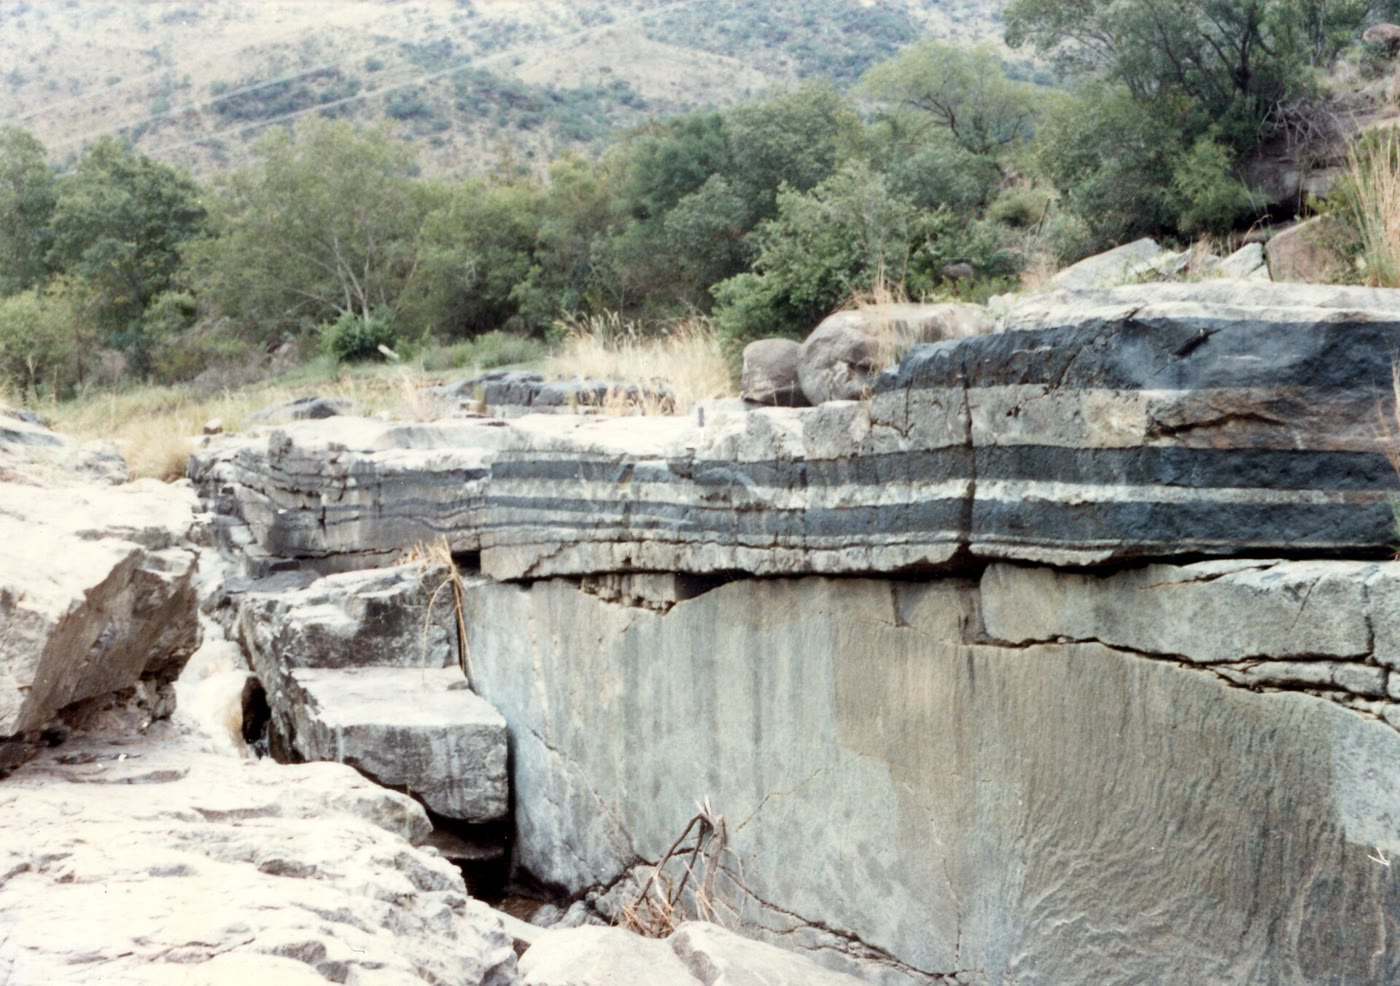
\includegraphics[height=5.2cm]{images/book4/b2-bushveld-chromitite.jpg}
\end{minipage}\hfill
\begin{minipage}[t]{0.42\linewidth}\vspace{0pt}\centering
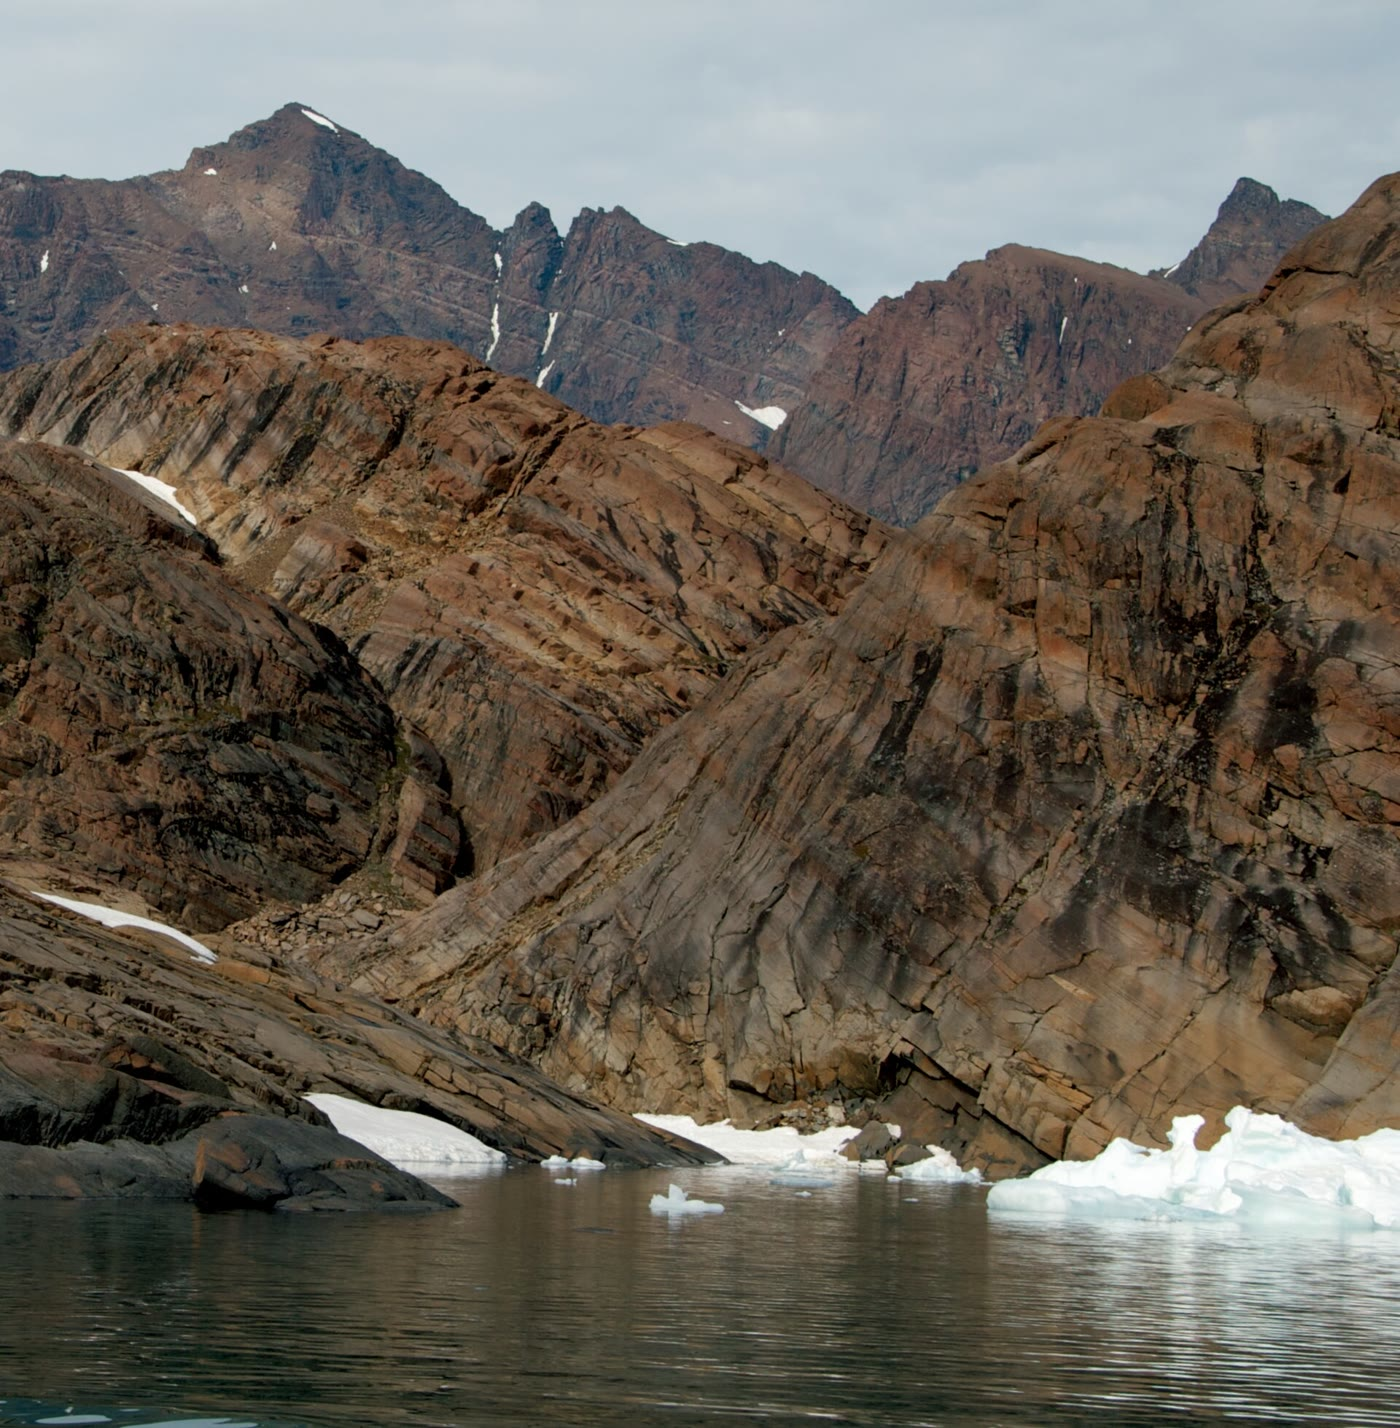
\includegraphics[height=5.2cm]{images/book4/b2-skaergaard-layering.jpg}
\end{minipage}
\par\smallskip{\small À gauche~: couches de chromitite noire et d'anorthosite grise de la zone critique
du complexe du Bushveld, Afrique du Sud (Kevin Walsh, CC BY 2.0). À droite~: les gabbros lités de la zone
moyenne de l'intrusion de Skaergaard, est du Groenland, inclinés du haut à gauche vers le bas à droite
(C. Tegner, CC BY 4.0).}
\end{omfigure}

\section{Systèmes ouverts}\label{sec:b2:magmatic-differentiation:open}

Une chambre magmatique est rarement fermée. Du \omterm{def:b2:magma-emplacement:magma}{magma} neuf arrive par le bas, et les parois de la
chambre sont des roches que le \omterm{def:b2:magma-emplacement:magma}{magma} peut chauffer, fondre et dissoudre.

\begin{definition}[Mélange de magmas~; assimilation crustale~; AFC]
\label{def:b2:magmatic-differentiation:open}
Le \emph{mélange de magmas}\index{mélange de magmas} est l'homogénéisation de deux \omterm{def:b2:magma-emplacement:magma}{magmas} de
compositions différentes en un seul. L'\emph{assimilation crustale}\index{assimilation crustale} est
l'incorporation de roche crustale dans un \omterm{def:b2:magma-emplacement:magma}{magma}, par fusion
et dissolution de la roche des parois ou de blocs tombés dans celui-ci.
L'\emph{assimilation--cristallisation fractionnée}\index{assimilation--cristallisation fractionnée}
(AFC) est leur combinaison dans une même chambre~: le \omterm{def:b2:magma-emplacement:magma}{magma}
cristallise, et la chaleur latente libérée fond et assimile la roche des parois.
\end{definition}

\begin{proposition}[Le mélange est linéaire en concentrations]\label{prop:b2:magmatic-differentiation:mixing}
Un mélange d'une fraction massique $s$ de \omterm{def:b2:magma-emplacement:magma}{magma} A et de $1-s$ de \omterm{def:b2:magma-emplacement:magma}{magma} B a pour concentration
$C = sC_A + (1-s)C_B$~: sur tout diagramme d'une concentration en fonction d'une
autre, les mélanges se placent sur le segment droit de A à B, et la règle des leviers donne
$s$.
\end{proposition}

\begin{proof}
Chaque élément se conserve~: $C(m_A + m_B) = m_AC_A + m_BC_B$~; diviser par $m_A + m_B$.
\end{proof}

Le mélange et le retrait de cristaux tracent tous deux des droites sur les \omterm{def:b2:magmatic-differentiation:harker}{diagrammes de Harker}~; les rapports
isotopiques permettent de les distinguer. La cristallisation ne modifie pas un rapport isotopique, alors que le
mélange avec une roche de rapport différent le modifie, le long de l'hyperbole de
\cref{ch:b2:isotope-geochemistry}. Une hausse de $^{87}$Sr/$^{86}$Sr avec la silice dans une suite
volcanique est donc la marque d'une assimilation.

\begin{proposition}[Assimilation avec cristallisation fractionnée]
\label{prop:b2:magmatic-differentiation:afc}
Un \omterm{def:b2:magma-emplacement:magma}{magma} cristallise des cristaux de coefficient de partage global $D$ pour un élément
et assimile une roche de paroi de concentration $C_a$ à un taux $r$ fois le taux de
cristallisation ($r \ne 1$). Avec $F$ la masse de \omterm{def:b2:magma-emplacement:magma}{magma} rapportée à sa masse initiale
et $z = (r + D - 1)/(r - 1)$,
\[
\frac{C}{C_0} = F^{-z} + \frac{r}{r - 1 + D}\,\frac{C_a}{C_0}\,\bigl(1 - F^{-z}\bigr).
\]
Pour $r = 0$, on retrouve la loi de Rayleigh. Le rapport isotopique de l'élément dans le \omterm{def:b2:magma-emplacement:magma}{magma}
est la moyenne de celui du \omterm{def:b2:magma-emplacement:magma}{magma} initial et de celui de la roche de paroi, pondérée par les deux
termes de cette somme.
\end{proposition}

\begin{proof}
Par unité de masse initiale, quand une masse $\mathrm dm_c$ cristallise, une masse
$r\,\mathrm dm_c$ est assimilée et la masse de \omterm{def:b2:magma-emplacement:magma}{magma} varie de $\mathrm dM =
-(1-r)\,\mathrm dm_c$. Le bilan de l'élément s'écrit $\mathrm d(MC) = rC_a\,\mathrm dm_c -
DC\,\mathrm dm_c$. En développant le membre de gauche et en remplaçant $\mathrm dm_c$ par
$-\mathrm dM/(1-r)$,
\[
M\frac{\mathrm dC}{\mathrm dM} = -C - \frac{rC_a - DC}{1-r}
= \frac{(r - 1 + D)\,C - rC_a}{1 - r} = -z\,\bigl(C - C^*\bigr),
\qquad C^* = \frac{rC_a}{r - 1 + D}.
\]
Donc $\mathrm d(C - C^*)/(C - C^*) = -z\,\mathrm dM/M$, et $C - C^*$ est proportionnel
à $M^{-z}$~; avec $C = C_0$ pour $M = 1$, on obtient $C = C^* + (C_0 - C^*)F^{-z}$, qui est la
formule. Pour $r = 0$, $z = 1 - D$ et $C^* = 0$. Les atomes issus du
\omterm{def:b2:magma-emplacement:magma}{magma} initial obéissent à la même équation avec $C_a = 0$, donc leur concentration vaut
$C_0F^{-z}$~; les autres proviennent de la paroi, d'où la pondération des rapports isotopiques.
\end{proof}

DePaolo a donné ces équations en 1981~; elles constituent le modèle standard d'un \omterm{def:b2:magma-emplacement:magma}{magma} contaminé
sur son trajet à travers la croûte. Elles cachent une contrainte thermique. La chaleur
nécessaire pour assimiler la roche vient de la chaleur latente des cristaux~: chauffer la croûte de 150 à
\qty{1150}{\celsius} demande environ \qty{1}{kJ/g}, la fondre \qty{300}{J/g}, alors que cristalliser
le \omterm{def:b2:magma-emplacement:magma}{magma} en libère environ \qty{400}{J/g}~; il faut donc qu'environ \qty{3.25}{g} de \omterm{def:b2:magma-emplacement:magma}{magma} cristallisent
pour chaque gramme de roche assimilée, et $r$ est bien inférieur à 1.
Wilcox a fait le même calcul pour le Parícutin~: ses \qty{25.4}{g} de monzonite quartzique, pris vers
\qty{200}{\celsius}, demandaient environ \qty{31350}{J} pour être
chauffés à \qty{1100}{\celsius} et fondus, la chaleur de cristallisation d'environ
\qty{85}{g} de plagioclase, bien plus que les \qty{12.5}{g} de cristaux que son bilan de
masse retirait. Le \omterm{def:b2:magma-emplacement:magma}{magma} éruptif ne pouvait pas payer lui-même son assimilation~:
la chaleur a dû provenir d'un volume de \omterm{def:b2:magma-emplacement:magma}{magma} plus grand que celui qui est entré en éruption,
cristallisant hors de vue (\cref{exo:b2:magmatic-differentiation:11}).
% ledger: depaolo81:afc, white09:afc-heat, wilcox54:heat, wilcox54:mass-balance

\begin{omfigure}
\centering
\begin{tikzpicture}
\begin{axis}[omrecord, name=left, width=0.47\linewidth, height=5.4cm,
  xmin=0.3, xmax=1, ymin=0.3, ymax=1.05, x dir=reverse,
  xlabel={magma restant $F$}, ylabel={Sr~: $C/C_0$},
  tick label style={font=\scriptsize}, label style={font=\small}]
\addplot[thick, black] table[x=F, y=srC_r0] {figdata/out/bachelor-2-differentiation-afc.dat};
\addplot[thick, blue!70!black] table[x=F, y=srC_r02] {figdata/out/bachelor-2-differentiation-afc.dat};
\addplot[thick, red!70!black] table[x=F, y=srC_r05] {figdata/out/bachelor-2-differentiation-afc.dat};
\end{axis}
\begin{axis}[omrecord, at={(left.east)}, anchor=west, xshift=1.7cm,
  width=0.47\linewidth, height=5.4cm,
  xmin=0.3, xmax=1, ymin=0.703, ymax=0.716, x dir=reverse,
  xlabel={magma restant $F$}, ylabel={$^{87}$Sr/$^{86}$Sr},
  y tick label style={/pgf/number format/fixed, /pgf/number format/precision=3},
  legend style={font=\scriptsize, at={(0.03,0.97)}, anchor=north west},
  tick label style={font=\scriptsize}, label style={font=\small}]
\addplot[thick, black] table[x=F, y=iso_r0] {figdata/out/bachelor-2-differentiation-afc.dat};
\addlegendentry{$r = 0$}
\addplot[thick, blue!70!black] table[x=F, y=iso_r02] {figdata/out/bachelor-2-differentiation-afc.dat};
\addlegendentry{$r = 0.2$}
\addplot[thick, red!70!black] table[x=F, y=iso_r05] {figdata/out/bachelor-2-differentiation-afc.dat};
\addlegendentry{$r = 0.5$}
\end{axis}
\end{tikzpicture}
\par\smallskip{\small Assimilation avec \omterm{def:b2:magmatic-differentiation:crystallisation}{cristallisation fractionnée} pour le strontium
($D = 1.5$, roche de paroi ayant la moitié du strontium du \omterm{def:b2:magma-emplacement:magma}{magma} et
$^{87}$Sr/$^{86}$Sr = 0.7200, \omterm{def:b2:magma-emplacement:magma}{magma} 0.7035~; valeurs illustratives). À gauche~: la
concentration baisse d'autant plus vite que le taux d'assimilation $r$ augmente, car la roche de paroi apporte
moins de strontium et davantage de cristaux se forment pour un même $F$. À droite~: le rapport isotopique,
inchangé par la seule cristallisation ($r = 0$), monte vers celui de la paroi.}
\end{omfigure}

\section{Lire les cristaux zonés}\label{sec:b2:magmatic-differentiation:zoning}

\begin{definition}[Zonation chimique]\label{def:b2:magmatic-differentiation:zoning}
Un cristal d'une solution solide présente une \emph{zonation chimique}\index{zonation chimique}
lorsque sa composition varie du cœur à la bordure, enregistrant le liquide changeant
dont sont issues les couches successives. La zonation est \emph{normale} lorsque la bordure est plus riche en
composant de basse température (le sodium dans le plagioclase), \emph{inverse} lorsqu'elle est
plus riche en celui de haute température, et \emph{oscillatoire} lorsqu'elle alterne.
\end{definition}

Un cristal zoné est une \omterm{def:b2:magmatic-differentiation:crystallisation}{cristallisation fractionnée} surprise en flagrant délit~: son cœur ne s'est pas
rééquilibré avec le liquide ultérieur. La figure ci-dessous calcule, sur la courbe de Bowen,
le plagioclase qui croît à partir d'un liquide à \qty{50}{\percent} d'anorthite. À
l'équilibre, les cristaux restent homogènes et finissent à \qty{50}{\percent}~; en \omterm{def:b2:magmatic-differentiation:crystallisation}{cristallisation fractionnée} parfaite,
chaque nouvelle couche est en équilibre avec un liquide toujours plus sodique,
et la bordure des derniers cristaux est presque de l'albite pure. La zonation normale, du cœur
calcique à la bordure sodique, est ce que prédit la série de Bowen pour un \omterm{def:b2:magma-emplacement:magma}{magma} en refroidissement.
Une zone inverse, une bande calcique à l'extérieur d'une zone sodique, indique que le cristal a été
brusquement baigné dans un liquide plus chaud ou plus calcique~: souvent l'arrivée d'un \omterm{def:b2:magma-emplacement:magma}{magma} neuf,
qui se mélange dans la chambre.
% ledger: bowen13:plagioclase, earle:bowen (Book 2)

\begin{omfigure}
\centering
\begin{tikzpicture}
\begin{axis}[omrecord, width=0.78\linewidth, height=6cm,
  xmin=0, xmax=1, ymin=0, ymax=90,
  xlabel={fraction du liquide cristallisé},
  ylabel={anorthite (\unit{\percent}, molaire)},
  legend style={font=\scriptsize, at={(0.02,0.02)}, anchor=south west},
  tick label style={font=\scriptsize}, label style={font=\small}]
\addplot[very thick, red!70!black] table[x=x, y=an_frac] {figdata/out/bachelor-2-differentiation-zoning.dat};
\addlegendentry{fractionnée~: couche en formation}
\addplot[thick, gray, densely dotted] table[x=x, y=an_liq_frac] {figdata/out/bachelor-2-differentiation-zoning.dat};
\addlegendentry{fractionnée~: liquide}
\addplot[very thick, blue!70!black, dashed] table[x=x, y=an_eq] {figdata/out/bachelor-2-differentiation-zoning.dat};
\addlegendentry{équilibre~: cristaux}
\end{axis}
\end{tikzpicture}
\par\smallskip{\small Plagioclase cristallisant à partir d'un liquide à \qty{50}{\percent}
d'anorthite, calculé sur la courbe de Bowen (1913). En \omterm{def:b2:magmatic-differentiation:crystallisation}{cristallisation fractionnée}, les couches
successives des cristaux, du cœur (à gauche) à la bordure (à droite),
deviennent de plus en plus sodiques,
et le liquide atteint l'albite lorsque environ \qty{82}{\percent} a cristallisé~; à l'équilibre,
les cristaux restent uniformes et finissent avec la composition du liquide dont ils sont issus.}
\end{omfigure}

\begin{inthelab}[Lire les cristaux zonés]
Les pétrologues lisent d'abord la zonation entre polariseurs croisés, où les zones d'un
plagioclase s'éteignent sous des angles légèrement différents et apparaissent en bandes concentriques.
Ils la mesurent ensuite~: une microsonde électronique (\cref{ch:b2:field-lab-methods-2})
analyse des points de quelques micromètres de large le long d'un profil du cœur à la bordure, et des cartes
du calcium et du sodium montrent directement les zones. À partir d'un tel profil, ils calculent
la composition du liquide dont chaque zone est issue, avec la courbe de la figure ci-dessus
ou avec des coefficients de partage, et ils comptent les zones inverses comme autant de
recharges de la chambre. Les \omterm{def:b2:elements-in-the-earth:trace}{éléments en traces} mesurés le long du même profil par ablation laser,
et les rapports isotopiques mesurés zone par zone, distinguent la cristallisation, le mélange
et l'assimilation dans l'histoire d'un seul cristal.
\end{inthelab}

\section{Exercices}

\begin{exercise}[$\star$]\label{exo:b2:magmatic-differentiation:1}
Utiliser les mesures de Bowen sur les plagioclases (solidus / liquidus, \unit{\celsius})~:
An$_{100}$ 1550 / 1550~; An$_{83.3}$ 1465 / 1521~; An$_{66.7}$ 1372 / 1490~; An$_{50}$
1287 / 1450~; An$_{33.3}$ 1205 / 1394~; An$_{20}$ liquidus 1334~; An$_{11.1}$ liquidus
1265, et interpoler linéairement entre les points voisins. Un liquide à
\qty{50}{\percent} d'anorthite se refroidit à l'équilibre. (a) À quelle température commence-t-il
à cristalliser, et quelle est la composition du premier cristal~? (b) À
\qty{1394}{\celsius}, quelles sont les compositions du liquide et des cristaux, et quelle fraction
massique a cristallisé (utiliser les fractions molaires comme si c'étaient des fractions massiques)~?
(c) Quelle est la composition de la dernière goutte de liquide~?
\end{exercise}
% ledger: bowen13:plagioclase

\begin{exercise}[$\star$]\label{exo:b2:magmatic-differentiation:2}
Un \omterm{def:b2:magmatic-differentiation:cumulate}{cumulat} gabbroïque contient \qty{50}{\percent} de plagioclase, \qty{35}{\percent}
de clinopyroxène et \qty{15}{\percent} d'olivine. Avec les coefficients de partage
(olivine / clinopyroxène / plagioclase) Sr 0.000063 / 0.157 / 2.7, Zr 0.00068 /
0.195 / 0.001 et Rb 0.000044 / 0.0033 / 0.025,
calculer le coefficient de partage global de chaque élément, et dire lequel est compatible.
\end{exercise}
% ledger: white07:kd-basalt

\begin{exercise}[$\star$]\label{exo:b2:magmatic-differentiation:3}
Le \omterm{def:b2:magmatic-differentiation:cumulate}{cumulat} de l'\cref{exo:b2:magmatic-differentiation:2} cristallise à partir d'un basalte, par \omterm{def:b2:magmatic-differentiation:crystallisation}{cristallisation fractionnée},
jusqu'à ce qu'il reste la moitié du liquide. (a) De quel facteur chacun de Sr, Zr et Rb a-t-il changé
dans le liquide (prendre les coefficients globaux 1.40, 0.069 et 0.014)~? (b) De quel facteur le rapport Zr/Rb a-t-il changé~?
Commenter à l'aide du corollaire sur les rapports.
\end{exercise}
% ledger: white07:kd-basalt

\begin{exercise}[$\star$]\label{exo:b2:magmatic-differentiation:4}
La première lave du Parícutin (février 1943) contenait \qty{55.04}{\percent} \ce{SiO2},
\qty{5.68}{\percent} \ce{MgO} et \qty{0.85}{\percent} \ce{K2O}~; la dernière (février
1952), 60.07, 3.73 et \qty{1.67}{\percent}. (a) Calculer la variation de chaque oxyde.
(b) La potasse n'entre dans aucun des minéraux qui cristallisent. Si elle s'était concentrée par
\omterm{def:b2:magmatic-differentiation:crystallisation}{cristallisation fractionnée} seule, quelle fraction du liquide serait restée~? (c) Le bilan de masse de Wilcox
ne retire qu'environ \qty{12.5}{g} de cristaux pour
\qty{100}{g} de \omterm{def:b2:magma-emplacement:magma}{magma}. Qu'est-ce que la comparaison suggère~?
\end{exercise}
% ledger: wilcox54:table2, wilcox54:mass-balance

\begin{exercise}[$\star\star$]\label{exo:b2:magmatic-differentiation:5}
Comparer \omterm{def:b2:magmatic-differentiation:crystallisation}{cristallisation fractionnée} et \omterm{def:b2:magmatic-differentiation:crystallisation}{cristallisation à l'équilibre}~: calculer $C_L/C_0$ par les deux lois
(a) pour le nickel, $D = 5$, lorsque \qty{20}{\percent} du liquide a cristallisé~; (b)
pour un \omterm{def:b2:elements-in-the-earth:partition}{élément incompatible}, $D = 0.01$, lorsque \qty{90}{\percent} a cristallisé.
(c) Quelles sont les limites des deux lois lorsque $F \to 0$~?
Quelle loi peut épuiser complètement un liquide en \omterm{def:b2:elements-in-the-earth:partition}{élément compatible}~?
\end{exercise}

\begin{exercise}[$\star\star$]\label{exo:b2:magmatic-differentiation:6}
(a) Calculer les pourcentages massiques de \ce{MgO}, \ce{FeO} et \ce{SiO2} dans l'olivine
Fo$_{80}$, $(\ce{Mg}_{0.8}\ce{Fe}_{0.2})_2\ce{SiO4}$ ($M$ = 40.30, 71.84 et
\qty{60.08}{g/mol}). (b) Un basalte à \qty{10.0}{\percent} de \ce{MgO} et
\qty{49.0}{\percent} de \ce{SiO2} ne cristallise que cette olivine jusqu'à ce que son liquide ait
\qty{8.0}{\percent} de \ce{MgO}. Quelle fraction massique d'olivine a été retirée~? (c) Quelle
est alors la teneur en silice du liquide~?
\end{exercise}

\begin{exercise}[$\star\star$]\label{exo:b2:magmatic-differentiation:7}
Pour l'intrusion de Skaergaard, $F = \num{1.091e-7}H^2 - \num{5.9064e-4}H + 0.7678$.
(a) Calculer $F$ pour $H = 0$, 1000 et \qty{2000}{m}. (b) À quelle hauteur $F = 0$~?
(c) Quelle fraction du \omterm{def:b2:magma-emplacement:magma}{magma} avait cristallisé avant la formation de la base de la séquence du plancher
affleurante, et où pouvait-elle se trouver~?
\end{exercise}
% ledger: tegner23:skaergaard

\begin{exercise}[$\star\star$]\label{exo:b2:magmatic-differentiation:8}
Le long de la coupe de Skaergaard, le \omterm{def:b2:magmatic-differentiation:cumulate}{cumulat} médian contient \qty{177}{ppm} de Ni à
$F = 0.70$ (zone inférieure a), \qty{54}{ppm} à $F = 0.29$ (zone moyenne) et
\qty{6.2}{ppm} à $F = 0.17$ (zone supérieure a). (a) En supposant que les \omterm{def:b2:magmatic-differentiation:cumulate}{cumulats} contiennent
$D$ fois le nickel de leur liquide et que le liquide suit la loi de Rayleigh,
calculer le $D$ apparent entre les deux premiers niveaux.
(b) Faire de même entre les deux derniers. (c) Qu'est-ce qui peut faire varier le $D$ apparent~?
\end{exercise}
% ledger: data:b4-skaergaard

\begin{exercise}[$\star\star$]\label{exo:b2:magmatic-differentiation:9}
Vérifier la réponse de Wilcox~: \qty{100}{g} de pâte de la première lave (\ce{SiO2}
55.53, \ce{MgO} 4.66, \ce{K2O} \qty{0.88}{\percent}) plus \qty{25.4}{g} de xénolite moyen
(72.48, 0.77, 3.64) moins \qty{2.9}{g} d'olivine Fo$_{80}$ (39.19, 42.06, 0)
moins \qty{9.6}{g} de plagioclase An$_{70}$ (50.54, 0, 0). (a) Quelle masse reste-t-il~? (b) Calculer
son \ce{SiO2}, son \ce{MgO} et son \ce{K2O}, et comparer avec la pâte de la lave 19
(60.16, 3.19 et \qty{1.75}{\percent}). (c) Quel oxyde s'accorde le moins bien~?
\end{exercise}
% ledger: wilcox54:groundmass, wilcox54:xenoliths, wilcox54:mass-balance

\begin{exercise}[$\star\star\star$]\label{exo:b2:magmatic-differentiation:10}
Un \omterm{def:b2:magma-emplacement:magma}{magma} assimile de la roche de paroi à $r = 0.2$ en cristallisant, avec $D_{\ce{Sr}} =
1.5$, $C_a/C_0 = 0.5$, $^{87}$Sr/$^{86}$Sr initial = 0.7035 et roche de paroi 0.7200.
(a) Calculer $z$, $F^{-z}$ et $C/C_0$ à $F = 0.7$. (b) Comparer avec la \omterm{def:b2:magmatic-differentiation:crystallisation}{cristallisation fractionnée} pure au même $F$,
et expliquer la différence par la masse de cristaux formés dans chaque cas.
(c) Calculer le $^{87}$Sr/$^{86}$Sr du \omterm{def:b2:magma-emplacement:magma}{magma}.
\end{exercise}

\begin{exercise}[$\star\star\star$]\label{exo:b2:magmatic-differentiation:11}
Suivre le bilan thermique de Wilcox pour le Parícutin. (a) Quelle quantité de chaleur un gramme de monzonite
quartzique doit-il recevoir pour passer de 200 à \qty{1100}{\celsius} (capacité thermique
\qty{1.1}{J/(g.K)}), puis pour fondre (\qty{250}{J/g})~? (b) Quelle quantité pour
\qty{25.4}{g}~? (c) Quelle masse de plagioclase An$_{70}$
(chaleur latente \qty{370}{J/g}) doit cristalliser pour la fournir~?
(d) Comparer aux \qty{12.5}{g} de cristaux du bilan de masse, calculer le rapport $r$ de l'assimilation à la cristallisation,
et dire ce que cela implique.
\end{exercise}
% ledger: wilcox54:heat, white09:afc-heat

\begin{exercise}[$\star\star\star$]\label{exo:b2:magmatic-differentiation:12}
Un basalte à \qty{250}{ppm} de Ni cristallise d'abord de l'olivine seule ($D = 5$) jusqu'à
$F = 0.8$, puis de l'olivine avec du plagioclase et du clinopyroxène (coefficient de partage global $D = 1.5$). (a) Calculer le facteur de variation
du nickel dans chaque étape, et la teneur en nickel du liquide à $F = 0.5$.
(b) Qu'aurait prédit une loi unique avec $D = 5$~?
(c) Expliquer pourquoi la loi de Rayleigh doit être appliquée par étapes.
\end{exercise}

\section{Problème~: l'intrusion qui a écrit sa propre histoire}

\begin{problem}[{Problème du week-end --- des couches d'un gabbro à la fraction de son magma
encore liquide à la fin}]
\label{pb:b2:magmatic-differentiation:1}
Un \omterm{def:b2:magma-emplacement:bodies}{sill} gabbroïque lité (fictif) a cristallisé à partir d'un basalte dont la marge figée
donne la composition du parent~: \ce{SiO2} 49.5, \ce{Al2O3} 16.0, \ce{FeO} 10.0,
\ce{MgO} 9.0, \ce{CaO} 11.5, \ce{Na2O} 2.5, \ce{K2O} \qty{0.30}{\percent}~;
\qty{150}{ppm} de Ni et \qty{80}{ppm} de Zr. Les \omterm{def:b2:magmatic-differentiation:cumulate}{cumulats} de la zone inférieure sont formés de
\qty{20}{\percent} d'olivine, \qty{50}{\percent} de plagioclase et \qty{30}{\percent}
de clinopyroxène~; au-dessus du niveau où l'olivine disparaît, de \qty{55}{\percent}
de plagioclase et \qty{45}{\percent} de clinopyroxène. Prendre les coefficients de partage
(olivine / plagioclase / clinopyroxène) Ni 5.0 / 0 / 2.0 et Zr 0.0007 / 0.001 /
0.195. Compositions des minéraux (\unit{\percent})~: olivine \ce{MgO} 42.06, \ce{CaO} 0,
\ce{Al2O3} 0, \ce{SiO2} 39.19~; plagioclase 0, 14.36, 31.70, 50.54~; clinopyroxène
16.0, 20.5, 3.0, 51.5. Un \omterm{def:b2:magma-emplacement:bodies}{dyke}
à grain fin, alimenté par la chambre lorsque la couche la plus haute a cristallisé, a pour composition
\ce{SiO2} 50.0, \ce{Al2O3} 14.1, \ce{FeO} 16.7, \ce{MgO} 4.9, \ce{CaO} 7.3,
\ce{Na2O} 3.4, \ce{K2O} \qty{0.75}{\percent} et \qty{188}{ppm} de Zr.

\noindent\textbf{Partie I --- Les coefficients de partage des couches.}
\begin{enumerate}
\item Calculer le coefficient de partage global du nickel dans la zone inférieure.
\item Calculer celui du zirconium dans la zone inférieure.
\item Calculer les deux dans la zone supérieure.
\item Quel élément est compatible dans chaque zone~? Le nickel reste-t-il compatible
quand l'olivine disparaît~?
\item Quel minéral porte l'essentiel du zirconium des \omterm{def:b2:magmatic-differentiation:cumulate}{cumulats}, et pourquoi~?
\item De quel facteur le rapport Ni/Zr du liquide change-t-il à chaque division par deux de $F$
dans la zone inférieure~?
\end{enumerate}

\noindent\textbf{Partie II --- Courbes de Rayleigh le long de la coupe.}
\begin{enumerate}[resume]
\item Quelle teneur en nickel attendez-vous dans le \omterm{def:b2:magmatic-differentiation:cumulate}{cumulat} le plus bas, cristallisé à
$F = 1$~?
\item Un \omterm{def:b2:magmatic-differentiation:cumulate}{cumulat} de la zone inférieure, plus haut, contient \qty{190}{ppm} de Ni. À quel $F$ s'est-il
formé~?
\item Quelle était alors la teneur en zirconium du liquide~?
\item À ce $F$, comparer le nickel du liquide donné par les lois
fractionnée et à l'équilibre.
\item L'olivine disparaît à $F = 0.55$. Calculer la teneur en nickel du liquide
à ce niveau.
\item Calculer le nickel des \omterm{def:b2:magmatic-differentiation:cumulate}{cumulats} formés juste au-dessous et juste au-dessus de ce
niveau. Quel trait un géologue verrait-il dans le profil~?
\item Calculer le nickel du liquide et du \omterm{def:b2:magmatic-differentiation:cumulate}{cumulat} à $F = 0.40$. Expliquer
la tendance.
\end{enumerate}

\noindent\textbf{Partie III --- Le bilan de masse du dernier liquide.}
\begin{enumerate}[resume]
\item Écrire l'équation de conservation de la méthode pour un oxyde, avec les masses
$x_{\mathrm{ol}}, x_{\mathrm{pl}}, x_{\mathrm{cpx}}$ retirées pour \qty{100}{g} de
parent et le \omterm{def:b2:magma-emplacement:bodies}{dyke} comme fils.
\item L'écrire pour \ce{MgO}, \ce{CaO} et \ce{Al2O3}.
\item Résoudre le système $3 \times 3$.
\item Quelle fraction du parent reste à l'état de liquide~?
\item Vérifier la réponse avec \ce{SiO2}~: recalculer la silice du liquide à partir des
masses trouvées.
\item Comparer les proportions des minéraux retirés aux modes des deux
zones.
\item La potasse n'entre dans aucun des minéraux~: quelle fraction de liquide donne-t-elle~?
\end{enumerate}

\noindent\textbf{Partie IV --- La fraction de liquide au sommet.}
\begin{enumerate}[resume]
\item De quel facteur le zirconium avait-il augmenté dans le liquide lorsque l'olivine disparut à
$F = 0.55$~? Donner alors la teneur en zirconium.
\item À partir du zirconium du \omterm{def:b2:magma-emplacement:bodies}{dyke}, calculer la fraction de liquide restant au moment de sa
formation, en appliquant la loi de la zone supérieure à partir de $F = 0.55$.
\item Refaire le calcul avec un seul $D = 0.07$ depuis le début. La réponse est-elle
sensible aux détails de $D$~?
\item Le fer est passé de 10.0 à \qty{16.7}{\percent} dans le liquide, alors que la silice a à peine
changé. Quels minéraux en sont responsables, et quel type de série magmatique
cela annonce-t-il (\cref{ch:b2:magmatic-series})~?
\item Les \omterm{def:b2:magmatic-differentiation:cumulate}{cumulats} les plus hauts contiennent \qty{47}{ppm} de Zr. Les seuls cristaux cumulus contiendraient
$\bar D$ fois le zirconium du liquide~; quelle fraction massique de liquide piégé
(de composition du \omterm{def:b2:magma-emplacement:bodies}{dyke}) explique l'analyse~?
\item Donner la fraction du \omterm{def:b2:magma-emplacement:magma}{magma} d'origine encore liquide lorsque la couche la plus haute
a cristallisé, le nombre clé de ce problème, et comparer les trois estimations
(éléments majeurs, potasse, zirconium).
\end{enumerate}
\end{problem}
% ledger: white07:kd-basalt, matzen12:dni
